\documentclass{article}
\usepackage[margin=1in]{geometry}
\usepackage{graphicx}
\usepackage{tikz}
\usetikzlibrary{arrows}

\newcommand{\vect}[1]{\left\langle #1 \right\rangle}
\begin{document}
\noindent{\large \bf Solutions}
\noindent{\bf CSCI 480, Fall 2015, Math Homework \# 2}

\begin{enumerate}

\item
  In the picture below, $a$, $b$, and $c$ are arbitrary points, and
  the dotted line from $b$ to $x$ is perpendicular to the line from
  $a$ to $c$.  Give formulas to find each of the
  distances from 
  $a$, $b$, and $c$ to $x$ as a function of the points $a$, $b$, and $c$.
  Use point subtraction and dot products.  Each formula should stand
  on its own and not depend on the other formulas.

\newcommand{\mypoint}[3] {
  \node (#1) at (#2) {};
  \fill (#2) circle (2pt);
  \node[anchor=#3] (label#1) at (#2) {$#1$};
  }
\begin{tikzpicture}
%  \draw[help lines] (0,0) grid (8,5);
  \mypoint{a}{1,3}{east};
  \mypoint{b}{5,5}{south};
  \mypoint{c}{8,1}{west};
  \mypoint{x}{4.2,2.1}{north};
\draw (a) -- (b) -- (c) -- (a);
\draw[dotted] (b) -- (x);
\end{tikzpicture}

\begin{description}
\item[Distance $a$ to $x$:]
  Normal vector from $a$ pointing at $c$:
  \[ \frac{c-a}{|c-a|} \]
  Distance from $a$ to $x$ is given by the projection of $b-a$
  onto $c-a$: \[ (b-a) \cdot \frac{c-a}{|c-a|} \]

\item[Distance $b$ to $x$:] Use Pythagoras formula with the distances
  between $a$ and $b$ and $a$ and $x$:
  \[
  \sqrt{|a-b|^2 - \left((b-a) \cdot \frac{c-a}{|c-a|} \right)^2}
  \]

  

\item[Distance $c$ to $x$:]
  Similar to distance $a$ to $x$:
  \[ (b-c) \cdot \frac{a-c}{|a-c|} \]
 
  
\end{description}



\item For each of the following implicitly defined quadric surfaces,
  find fomulas for  the coefficients  for the quadratic equation,
  $at^2 + bt + c = 0$
  to determine the value of $t$ where a ray defined by $p + tv$
  intersects the surface. 
  \begin{enumerate}
  \item Elliptic paraboloid \[\frac{x^2}{a^2} + \frac{y^2}{b^2} - z =
    0\]
\begin{eqnarray*}
\frac{(p_x +tv_x)^2}{a^2} +\frac{(p_y +tv_y)^2}{b^2} - (p_z +tv_z)
&=&
\left(\frac{v_x^2}{a^2} + \frac{v_y^2}{b^2}\right)t^2
+
\left(\frac{2v_x}{a^2} + \frac{2v_y}{b^2} - v_z\right)t
+
\left(\frac{p_x^2}{a^2} + \frac{p_y^2}{b^2} - {p_z}\right)
\\
a&=&\left(\frac{v_x^2}{a^2} + \frac{v_y^2}{b^2}\right)t^2\\
b&=&\left(\frac{2v_x}{a^2} + \frac{2v_y}{b^2} - v_z\right)\\
c&=&\left(\frac{p_x^2}{a^2} + \frac{p_y^2}{b^2} - {p_z}\right)
\end{eqnarray*}

\item Hyperbolic paraboloid \[\frac{x^2}{a^2} - \frac{y^2}{b^2} - z\ = 0\]
  \begin{eqnarray*}
a&=&\left(\frac{v_x^2}{a^2} - \frac{v_y^2}{b^2}\right)t^2\\
b&=&\left(\frac{2v_x}{a^2} - \frac{2v_y}{b^2} - v_z\right)\\
c&=&\left(\frac{p_x^2}{a^2} - \frac{p_y^2}{b^2} - {p_z}\right)
\end{eqnarray*}


\item Elliptic hyperboloid of one sheet
  \[\frac{x^2}{a^2} + \frac{y^2}{b^2} - \frac{z^2}{c^2}\ = 1\]
  \begin{eqnarray*}
a&=&\left(\frac{v_x^2}{a^2} + \frac{v_y^2}{b^2} - \frac{v_z^2}{c^2}\right)t^2\\
b&=&\left(\frac{2v_x}{a^2} + \frac{2v_y}{b^2} - \frac{2v_z}{c^2}\right)\\
c&=&\left(\frac{p_x^2}{a^2} + \frac{p_y^2}{b^2} - \frac{p_z^2}{c^2}\right)-1
\end{eqnarray*}
  

  \item Elliptic hyperboloid of two sheets
    \[ \frac{x^2}{a^2} + \frac{y^2}{b^2} - \frac{z^2}{c^2} = -1\]
  \begin{eqnarray*}
a&=&\left(\frac{v_x^2}{a^2} + \frac{v_y^2}{b^2} - \frac{v_z^2}{c^2}\right)t^2\\
b&=&\left(\frac{2v_x}{a^2} + \frac{2v_y}{b^2} - \frac{2v_z}{c^2}\right)\\
c&=&\left(\frac{p_x^2}{a^2} + \frac{p_y^2}{b^2} - \frac{p_z^2}{c^2}\right)+1
\end{eqnarray*}
  \end{enumerate}
  
  
\item Find a formula for a vector normal to each of the following
  surfaces, given a point $(x,y,z)$ on the surface.
  \begin{enumerate}
  \item Elliptic paraboloid \[\frac{x^2}{a^2} + \frac{y^2}{b^2} - z = 0\]
    \[
    \nabla f(x,y,z) = \vect{\frac{2x}{a^2}, \frac{2y}{b^2}, -1}
    \]

  \item Hyperbolic paraboloid \[\frac{x^2}{a^2} - \frac{y^2}{b^2} - z\ = 0\]
    \[
    \nabla f(x,y,z) = \vect{\frac{2x}{a^2}, \frac{-2y}{b^2}, -1}
    \]

  \item Elliptic hyperboloid of one sheet
    \[\frac{x^2}{a^2} + \frac{y^2}{b^2} - \frac{z^2}{c^2}\ = 1\]
    \[
    \nabla f(x,y,z) = \vect{\frac{2x}{a^2}, \frac{2y}{b^2}, \frac{-2z}{c^2}}
    \]

  \item Elliptic hyperboloid of two sheets
    \[ \frac{x^2}{a^2} + \frac{y^2}{b^2} - \frac{z^2}{c^2} = -1\]
    \[
    \nabla f(x,y,z) = \vect{\frac{2x}{a^2}, \frac{2y}{b^2}, \frac{-2z}{c^2}}
    \]

  \end{enumerate}

\item Suppose we specify a camera by five points: the eye point and the four corners of
  the image plane (upper left, upper right, lower left, lower right),
  as in the figure below (the left side of the image plane is deeper
  into the picture than the right side). 

    \tikzset{>=latex}
    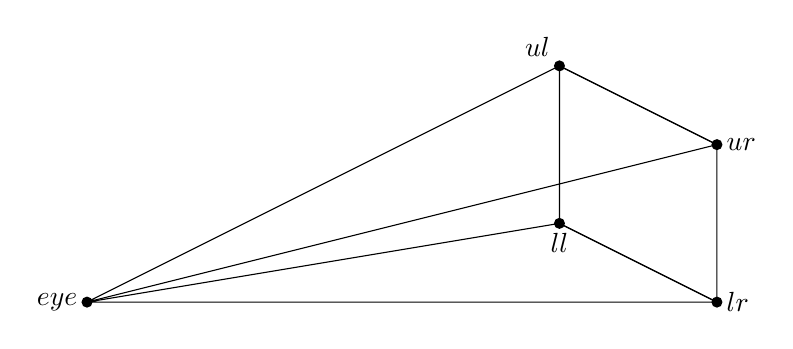
\begin{tikzpicture}
      \fill (1,2) circle (2pt) node[anchor=east] {$eye$};
      \fill (7,5) circle (2pt) node[anchor=south east] {$ul$};
      \fill (7,3) circle (2pt) node[anchor=north] {$ll$};
      \fill (9,4) circle (2pt) node[anchor=west] {$ur$};
      \fill (9,2) circle (2pt) node[anchor=west] {$lr$};

      \draw (1,2) -- (7,5) -- (9,4) -- cycle;
      \draw (1,2) -- (7,3) -- (9,2) -- cycle;
      \draw (7,3) -- (7,5) -- (9,4) -- (9,2) -- cycle;
    \end{tikzpicture}

Given a position in the image plane defined by $x$ and $y$, each
scaled to $[0,1]$, and with the origin of the image plane understood
as the lower left corner, write an expression giving the vector for a
ray from the eye to that point in the image plane.  You do not need to
normalize the vector.

\[ (ll + x(lr-ll) + y(ul-ll)) - eye\]

\item Given a camera specified as in the lecture notes, with an eye
  point, normalized right, up, and foward vectors, and scalars depth,
  width and height, $\langle p, r, u, f, d, w, h\rangle$, write
  expressions for each of the five points in the camera representation
  from the previous problem.
  \begin{enumerate}
  \item \[eye = eye\]

    \item \[ul =  eye + d(f) - (w/2) r + (h/2) u\]

    \item \[ur = eye + d(f) + (w/2) r + (h/2) u\]

    \item \[ll = eye + d(f) - (w/2) r - (h/2) u\]

    \item \[lr = eye + d(f) + (w/2) r - (h/2) u\]

  \end{enumerate}
  
\end{enumerate}
\end{document}
